\documentclass{article}

\usepackage[english]{babel}
\usepackage[margin=3cm]{geometry}
\usepackage{graphicx}
\usepackage{float}
\usepackage{caption}
\usepackage{hyperref}
\usepackage{amsmath}
\usepackage{wrapfig}
\usepackage[parfill]{parskip}

% fonts
\usepackage[T1]{fontenc}
\usepackage{helvet}
\renewcommand{\familydefault}{\sfdefault}

\graphicspath{{img/}}

% theorem environment
\usepackage{amssymb}

\newtheorem{theorem}{Definitie}[section]

\usepackage{enumitem}

\newenvironment{thmenum}
 {\begin{enumerate}[label=\upshape\bfseries(\roman*)]}
 {\end{enumerate}}


% code
\usepackage{minted}
\setminted{frame=single,framesep=3pt,linenos}
\usepackage{upquote}
\usepackage{color}

\begin{document}

\begin{titlepage}
    \author{Tuur Vanhoutte}
    \title{Linux OS}
\end{titlepage}

\pagenumbering{gobble}
\maketitle
\newpage
\tableofcontents
\newpage

\pagenumbering{arabic}

\section{Introductie}

\subsection{Verschil Server \& Workstation}

\subsubsection{Server}

\begin{itemize}
    \item Deliver services to (multiple) users
    \item Focussed: only this and nothing else
    \item Secure
    \item No GUI, everything happens through the commandline
    \item $\Rightarrow$ as small a footprint as possible
\end{itemize}

\subsubsection{Workstation}

\begin{itemize}
    \item Use services
    \item Create documents
    \item Look for information
    \item Consume multimedia
    \item GUI
    \item $\Rightarrow$ Large footprint
\end{itemize}

\subsection{Extra information/resources}

\begin{itemize}
    \item The Linux Documentation Project: \url{http://tldp.org}
    \item Pluralsight LPIC-1: Linux Professional Institute Certification: \url{https://www.pluralsight.com/paths/lpic-1}
    \item The Arch Linux Wiki is one of the most extensive sources of info about Linux: \url{https://wiki.archlinux.org}
    \begin{itemize}
        \item In this module we will use Debian, not Arch, but many things are very similar
    \end{itemize}
    \item Google
\end{itemize}

\subsection{What is Linux?}

\subsubsection{What is an operating system (OS)?}

\begin{theorem}[Operating System]
An operating system, or OS, is software that communicates with the hardware
and alows other programs to run. 

It is comprised of system software = the fundamental files your computer needs to function.
\end{theorem}


\textcolor{red}{Linux is NOT an operating system: Linux = the \underline{\textbf{kernel}}}

\subsubsection{What is a Kernel?}

\begin{theorem}[Kernel]
The kernel is software that is the core of a computer's operating system, with complete control over the system.

It is the first program loaded on start-up. 

It handles\dots: 

\begin{itemize}
    \item \dots the rest of the startup
    \item \dots input/output requests from software, translating them into instructions for the CPU
    \item \dots memory
    \item \dots peripherals
\end{itemize}
\end{theorem}


\subsection{GNU Operating System}

\begin{theorem}[GNU]
GNU = GNU's Not Unix (recursive algorithm)

Founded by Richard Stallman (ex-MIT, founder of the Free Software Foundation), 1984

Goal: completely free Operating System
\end{theorem}

\subsection{Linux, the kernel}

By Linus Torvalds (Finland), 1991

\begin{itemize}
    \item Own personal development, not initially intended to distribute
    \item Interest from other developers, mainly to use with GNU OS
    \item Meanwhile contributions of over 12000+ developers
    \item 492 of top-500 supercomputers in the world run Linux
    \item Basis for Android, Chrome OS
\end{itemize}

Linux = the kernel

GNU = OS-tools around the kernel

$\Rightarrow$ \textbf{GNU/Linux}

\subsubsection{Distributions}

\begin{theorem}[Distribution]
A Linux distribution (or distro for short) is GNU/Linux + extra tools and applications to create a full-fledged OS.

That distribution can be easily copied and installed to other computers.
\end{theorem}

\begin{itemize}
    \item RedHat (CentOS)
    \item Debian (Ubuntu)
    \item Arch Linux
    \item Void Linux
    \item Gentoo
    \item Pop! OS
\end{itemize}

\begin{figure}[H]
    \centering
    \includegraphics[width=0.75\textwidth]{redhat-vs-debian-tree.png}
    \caption{\url{https://upload.wikimedia.org/wikipedia/commons/1/1b/Linux_Distribution_Timeline.svg}}
\end{figure}

\url{https://en.wikipedia.org/wiki/List_of_Linux_distributions}

\subsection{Open Source}

\begin{theorem}[Open Source]
Open source software is software of which the code is licensed to be open to everyone. 

Anyone can use, change, distribute the software. This allows code to be developed in a public manner.
\end{theorem}

\textbf{\textcolor{red}{OPEN SOURCE DOES NOT MEAN FREE}}

\subsubsection{Commercial distributions}

= Open source, non-free distributions

\begin{itemize}
    \item SUSE Linux Enterprise Server (SLES)
    \item SUSE Linux Enterprise Desktop (SLED)
    \item Red Hat Enterprise Linux (RHEL)
    \item Oracle Enterprise Linux
\end{itemize}

Commercial distributions have official support channels.

$\Rightarrow$ You're not paying for the operating system, you're paying for the support.

\subsubsection{In this course: Debian}


\begin{itemize}
    \item Current version: 10.7
    \item Forms the basis of many others: Ubuntu, Raspbian, Knoppix, Linux Mint
    \item Available on many platforms: Intel x86, AMD64, Intel64, ARM, MIPS, Power Systems, \dots
\end{itemize}

\section{Debian Installation}

\textbf{See Labs for detailed Installation tutorial}

\subsection{Networking in Linux (with VMWare)}

\begin{itemize}
    \item VMWare presents ethernet adapter
    \item During creation of virtual machine: MAC-address is created
    \item During installation: network configuration through DHCP
    \begin{itemize}
        \item IPv4-address
        \item Default gateway
        \item DNS-server
        \item \underline{Optional:} proxy-server
    \end{itemize}
\end{itemize}

\subsection{Users in Linux}

\begin{itemize}
    \item Linux is multi-user from the ground up
    \begin{itemize}
        \item Multiple users can be active at the same time
    \end{itemize}
    \item `Administrator'-user is called root
    \item Each user has a user-ID (uid)
    \begin{itemize}
        \item root has uid=0
        \item uid=0 has all rights
    \end{itemize}
    \item Each user has a home-directory
\end{itemize}

\subsection{Disks, partition, filesystems}

\begin{itemize}
    \item Our VM has 1 disk
    \begin{itemize}
        \item Presented on the SCSI-bus
        \item First disk on SCSI-bus: \textbf{sda}
        \item Then sdb, sdc, \dots
    \end{itemize}
    \item Disk = concatenation of blocks
    \item Divide blocks in collections (=partitions)
    \begin{itemize}
        \item 1st partition: sda1
        \item 2nd partition: sda2
        \item \dots
    \end{itemize}
    \item 2 types of partitions
    \begin{itemize}
        \item Primary
        \item Extended
    \end{itemize}
\end{itemize}

\subsubsection{Partitions}

Primary partition

\begin{itemize}
    \item A filesystem can be created inside this
    \item Up to 4 primary partitions
\end{itemize}

Extended Partition

\begin{itemize}
    \item `Logical' partitions can be created inside this
\end{itemize}

Our setup:

\begin{itemize}
    \item sda1: primary partition
    \item sda2: extended partition
    \item sda5: `logical' partition inside extended partition sda2
\end{itemize}

\begin{figure}[H]
    \centering
    \includegraphics[width=0.3\textwidth]{partitions.png}
    \caption{Our setup}
\end{figure}

\subsection{MBR <> GPT}

\subsubsection{MBR}

We use the MBR Partitioning scheme

\begin{theorem}[MBR]
MBR, or Master Boot Record, is a special type of boot sector at the start of a disk.

It contains: 

\begin{itemize}
    \item a set of instructions necessary to boot operating systems.
    \item info about how partitions are placed on disk
\end{itemize}


\end{theorem}

Limitations:

\begin{itemize}
    \item Maximum disks of 2TB
    \item 32-bit for number of logical sectors
    \item Common sector size: 512 bytes
    \item $2^{32} \cdot 512\ \text{bytes} = 4294967296 \cdot 512\ \text{bytes} \approx 2\text{TB}$
\end{itemize}

BIOS can boot from a disk with MBR partitioning

\subsubsection{GPT}

\begin{theorem}[GPT]
GPT, or GUID Partition Table, is a standard for the layout of partition tables on a disk.
It's an alternative to MBR.

It uses unique identifiers (GUIDs) 
\end{theorem}

\begin{itemize}
    \item BIOS cannot boot from a disk with GPT-partitioning: UEFI required when using GPT
    \item GPT allows disks larger than 2TB
\end{itemize}

\begin{theorem}[UEFI]
UEFI, or Unified Extensible Firmware Interface, is a newer firmware interface by Intel (90's) that replaces the BIOS interface by IBM (70's).
\end{theorem}

\textbf{How does it work?}

\begin{itemize}
    \item Disk = collection of blocks
    \item Group of blocks together = sector
    \item Common sector size: 512 bytes
    \item Sectors indicated with Logical Block Addresses (LBA)
    \item MBR in LBA 0
    \item GPT headers in LBA 1
    \item Partition tabel right after that
\end{itemize}




\subsubsection{Bootstrap procedure}

\begin{enumerate}
    \item Motherboard gets electricity
    \item Mini-loader hardcoded in memory
    \begin{itemize}
        \item BIOS gets loaded
    \end{itemize}
    \item Boot media are consulted
    \item First boot medium, first sectors are being read $\Rightarrow$
    \item MBR contains a bit-more-advanced loader: GRUB
    \begin{itemize}
        \item \underline{GR}and \underline{U}nified \underline{B}ootloader
    \end{itemize}
    \item This loader loads a more advanced loader (GRUB second stage bootloader)
    \item The OS is loaded
\end{enumerate}

\subsubsection{Linux boot process}

6 high level steps

\begin{itemize}
    \item BIOS (Basic Input/Output System) - loads MBR
    \item MBR (Master Boot Record) - loads GRUB
    \item GRUB (Grand Unified Bootloader) - loads kernel
    \item Kernel - executes /sbin/init
    \item Init - executes runlevel programs
    \item Runlevel - programs from /etc/rc.d/rcXX.d are started
\end{itemize}

\subsubsection{BIOS <> UEFI}

\begin{itemize}
    \item Recent systems use UEFI, not BIOS
    \item UEFI is required to boot from GPT-disk
    \item Linux has no trouble working with UEFI
\end{itemize}

\textbf{So why will we use MBR?}

\begin{itemize}
    \item Virtualisation is the norm
    \item Virtual machines typically have small disks
    \item Small disks are MBR partitioned
\end{itemize}



\subsection{Filesystems}

\subsubsection{Windows}

\begin{itemize}
    \item FAT (1977)
    \item FAT32 (1996)
    \item NTFS (1993)
    \item ReFS (2012)
\end{itemize}

\subsubsection{Linux}

\begin{itemize}
    \item Ext (1992)
    \item Ext2 (1993)
    \item Ext3 (2001)
    \item Ext4 (2008)
    \item ZFS (2005)
    \item BtrFS (2007)
\end{itemize}

\subsubsection{Swap}

= Paging

\begin{itemize}
    \item Free up physical memory (RAM) by moving pages to slower storage (storage disks instead of RAM)
    \item Page out $=$ memory page moves to swap
    \item "Swapiness"
    \begin{itemize}
        \item = parameter between 0 and 100
        \item = how quickly linux will swap
        \begin{itemize}
            \item 0 = very conservative
            \item 100 = very agressive
        \end{itemize}
    \end{itemize}
    \item Windows uses a swap file (pagefile.sys)
    \item Linux uses a swap partition
\end{itemize}

\subsection{File structure}



\begin{figure}[H]
    \centering
    \includegraphics[width=0.4\textwidth]{linux-filestructure.png}
    \caption{Linux uses a tree structure}
\end{figure}

\begin{figure}[H]
    \centering
    \includegraphics[width=0.5\textwidth]{windows-filestructure.png}
    \caption{Windows uses a similar structure, but every volume uses a letter.}
\end{figure}

\begin{figure}[H]
    \centering
    \includegraphics[width=0.5\textwidth]{linux-filestructure2.png}
    \caption{With linux, volumes are `mounted' to folders somewhere under root /}
\end{figure}

\subsection{Configuration}

\subsubsection{Packages}

\begin{itemize}
    \item Tools and applications are build up by files
    \item All files belonging to 1 application are bundled in a package
    \item Packages in debian have the .deb extension
\end{itemize}

Repositories

\begin{itemize}
    \item Packages are collected in repositories
    \item Are made available through the internet
    \item Packages have dependencies
\end{itemize}

\subsubsection{Package management}

Debian: dpkg \& apt (Advanced Package Tool)

\begin{itemize}
    \item dpkg: Install, remove, give info about .deb packages
    \begin{itemize}
        \item dpkg -l = lists packages 
    \end{itemize}
    \item apt: Get packages from a repository and install, remove, give info, ...
    \begin{itemize}
        \item apt update
        \begin{itemize}
            \item Contact the repositories
            \item Get most recent list of packages and versions
        \end{itemize}
        \item apt upgrade
        \begin{itemize}
            \item Of the packages which are more recent in the repositories compared to what is installed: install newest version
        \end{itemize}
        \item apt install <xyz>
        \begin{itemize}
            \item Download package <xyz> from the repository
            \item Check the dependencies and download depending packages
            \item Install package <xyz> and all corresponding dependencies
        \end{itemize}
    \end{itemize}
\end{itemize}

Which repositories? See /etc/apt/sources.list for the list of repositories. You can add/remove/change repositories in this file.

\subsubsection{Useful packages}

\begin{itemize}
    \item open-vm-tools
    \item vim
    \item sudo
    \item tcpdump
\end{itemize}

Install multiple pacakges in one command: apt install vim sudo tcpdump ntp

\subsection{Shutdown of VM}

\begin{itemize}
    \item Power button (=ACPI shutdown)
    \item Shut down operating system only
    \begin{itemize}
        \item = halt
    \end{itemize}
    \item Shut down operating system and VM, multiple ways:
    \begin{itemize}
        \item shutdown -P now
        \item init 0
        \item poweroff
    \end{itemize}
    \item Reboot
    \begin{itemize}
        \item reboot
        \item init 6
        \item shutdown -r now
    \end{itemize}
\end{itemize}

\subsection{Basic network}

\begin{itemize}
    \item No GUI $\Rightarrow$
    \item Layer 1: Physical (VMWare virtual network)
    \item Layer 2: Datalink (Ethernet \& MAC address)
    \item Layer 3: Network (IPv4)
    \item Layer 4: Transport (Transport Control Protocol (TCP), User Datagram Protocol (UDP))
    \item Layer 5: Application (SSH, HTTP, \dots)
\end{itemize}

\subsubsection{Basic networking commands}

\begin{itemize}
    \item arp
    \item ping
    \item route
    \item bmon
\end{itemize}

\subsection{Services}

\begin{itemize}
    \item Processes that `listen' on the network
    \begin{itemize}
        \item TCP or UDP port
    \end{itemize}
    \item Overview of currently running / listening services: ss command
    \begin{itemize}
        \item ss -tulpn
        \item t: show TCP
        \item u: show UDP
        \item l: show listening
        \item p: show process ID
        \item n: no name-resolving
    \end{itemize} 
\end{itemize}

\subsection{Wooclap Questions}

\begin{itemize}
    \item Why do we talk about GNU/Linux?
    \item What is a kernel?
    \item What is the difference between Open Source and free?
    \item How is the Administrator user called? What is its uid?
    \item What is MBR?
    \item What are the limitations of MBR? (Solution?)
    \item What is swap? What is swappiness?
    \item What is a package?
    \item What is a repository?
    \item What is a dependency?
    \item What is a package manager?
    \item What is the difference between 'apt update' and 'apt upgrade'
    \item Which protocol makes the link between MAC address \& IP address?
    \item Which command gives you the current ARP-table?
    \item What are the 5 layers of the TCP/IP network model?
    \item How do you find the MAC-address of a network interface?
    \item Put Linux boot process in correct order (6 levels)
    \item What is a linux distribution?
\end{itemize}

\section{File structure}

\begin{itemize}
    \item Tree structure
    \begin{itemize}
        \item Leaves = files
        \item Branches = directories
        \item The tree is inverted, root = /
    \end{itemize}
    \item Everything is a file (even devices, random numbers, and RAM) under 1 root
    \item This is in contrast to Windows, where every volume is a root.
\end{itemize}

\begin{figure}[H]
    \centering
    \includegraphics[width=0.4\textwidth]{linux-filestructure.png}
    \caption{}
\end{figure}



\subsection{Intermezzo: single user mode}

\begin{itemize}
    \item Linux (the kernel) is built up as a multi-user system from the beginning
    \item Standard behaviour = multi-user
    \item But: also possible to boot in single-user mode
    \begin{itemize}
        \item No daemons, no multiple logins
        \item Sometimes called \textbf{Maintenance mode}
    \end{itemize}
    \item Examples of usage
    \begin{itemize}
        \item Filesystem repairs
        \item Upgrade of distribution
        \item Password recovery
        \item Adjustments to the root filesystem
        \item Forensics after security incident
    \end{itemize}
\end{itemize}

\subsubsection{Runlevels}

= predefined operating system status

\begin{itemize}
    \item Is presented with a number
    \item Linux has 7 runlevels:
    \begin{itemize}
        \item 0 = system halt (= VM shutdown)
        \item 1 = single user
        \item 2 = multi-user, no NFS (no network services, not often used)
        \item 3 = multi-user, CLI (Command Line Interface)
        \item 4 = self-definable
        \item 5 = multi-user, GUI (Graphical User Interface, if installed)
        \item 6 = reboot
    \end{itemize}
\end{itemize}

\subsection{Intermezzo: Add disk}

\textbf{Add a new disk without shutting down the system}

\begin{enumerate}
    \item Adjust VM: add disk
    \item Detect added disk
    \item Partition disk
    \begin{itemize}
        \item fdisk (for MBR)
        \item parted (for GPT)
    \end{itemize}
    \item Create filesystem
    \begin{itemize}
        \item Partition = collection of blocks (sectors)
        \item Not usable for the OS $\Rightarrow$ create filesystem
        \item mkfs.ext4 /dev/sdb1
        \begin{figure}[H]
            \centering
            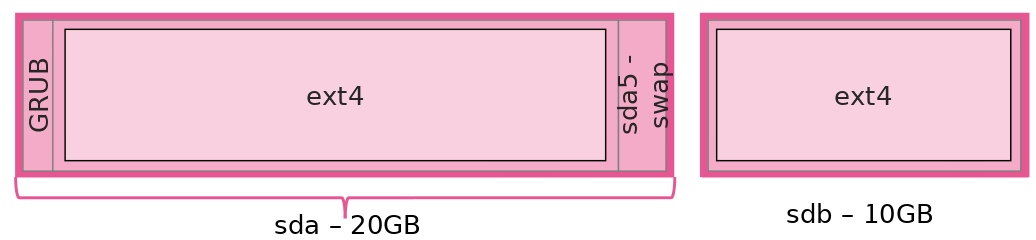
\includegraphics[width=0.7\textwidth]{create-filesystem.png}
            \caption{}
        \end{figure}
    \end{itemize}
    \item Mount filesystem
    \begin{itemize}
        \item mkdir /mnt/datadisk
        \item mount /dev/sdb1 /mnt/datadisk
        \item see if it worked: df -h
    \end{itemize}
\end{enumerate}

\textbf{For detailed steps: see labs!}


\subsubsection{What after a reboot?}

Use /etc/fstab = a file that contains what needs to be mounted at boot

\begin{itemize}
    \item Device (/dev/sdXY or UUID) 
    \item Mountpoint (/mnt/folder)
    \item Type of filesystem (ext4, ntfs, \dots)
    \item Options
\end{itemize}


\subsection{Navigate through the tree}

\begin{itemize}
    \item pwd
    \begin{itemize}
        \item Print working directory
        \item Shows where in the tree you are
    \end{itemize}
    \item ls
    \begin{itemize}
        \item Show a list of files in the working directory
        \item ls -la : 10 characters at the beginning of each line. The d == directory (see later)
    \end{itemize}
    \item When you login, you are in your home directory
    \item / (= the filesystem root) is not the same as /root (the home directory of the root user)
    \item . = current directory
    \item .. = the directory one higher
\end{itemize}

\subsubsection{Relative vs absolute path}

Relative paths:

\begin{itemize}
    \item cd .. = go to the directory above the current directory
    \item cat ../etc/issue = go to the etc directory, one directory above the current directory. Open the issue file
\end{itemize}

Absolute paths:

\begin{itemize}
    \item cd / = go to the root directory
    \item cat /etc/issue = go to the etc/ directory under / (root)
\end{itemize}

\subsection{Filesystem Hierarchy Standard (FHS)}

\begin{itemize}
    \item Describes how the filesystem in Linux is build up
    \item Maintained by the Linux Foundation
    \item Most recent version: v3.0 (2015)
\end{itemize}



\subsubsection{Rules in the standard}

\begin{itemize}
    \item / is the root of the tree structure
    \item /bin 
    \begin{itemize}
        \item essential binaries (executable files), required for single user mode
    \end{itemize}
    \item /boot
    \begin{itemize}
        \item the place on the filesystem where the boot files reside
        \item configuration files for GRUB
        \item kernels
        \item initrd
        \begin{itemize}
            \item initial RamDisk
            \item During boot a temporary root-filesystem is being created in RAM
            \item This is used so the kernel can load important modules, so it can then switch to the real root filesystem
            \item part of step 3 of the linux boot process (BIOS - MBR - GRUB - kernel - init - runlevel)
        \end{itemize}
    \end{itemize}
    \item /dev
    \begin{itemize}
        \item Devices get a place in the filesystem
        \begin{itemize}
            \item sda
            \item rtc
            \item random
            \item cpu
            \item urandom
            \item null
        \end{itemize}
        \item ls -lah /dev/
    \end{itemize}
    \item /etc
    \begin{itemize}
        \item Host-specific sytem-wide configuration files
        \item Configuration for this host, readable for the whole system
    \end{itemize}
    \item /home
    \begin{itemize}
        \item Each (non-system) user has a home directory
        \item except for root $\Rightarrow$ /root
    \end{itemize}
    \item /mnt
    \begin{itemize}
        \item (temporarily) `mounted' filesystems
        \begin{itemize}
            \item Network shares
            \item USB-disk
            \item DVD-ROM
            \item Extra disks
        \end{itemize}
        \item Some distributions use /media for this
    \end{itemize}
    \begin{figure}[H]
        \centering
        \includegraphics[width=0.3\textwidth]{linux-filestructure2.png}
        \caption{}
    \end{figure}
    
    \item /opt
    \begin{itemize}
        \item Optional application software packages
        \item Our installation $\Rightarrow$ no applications installed yet = empty (for now)
    \end{itemize}
    \item /proc
    \begin{itemize}
        \item Virtual filesystem
        \item Provides information about processes and the linux kernel
        \item cat /proc/cpuinfo
        \item cat /proc/sys/net/ipv4/ip\_forward
        \item cat /proc/partitions
    \end{itemize}
    \item /sbin
    \begin{itemize}
        \item Essential system binaries
        \item Only executable by root user
        \item fsck, init, route
    \end{itemize}
    \item /tmp
    \begin{itemize}
        \item Directory for temporary files
        \item Emptied at reboot (with most distributions)
    \end{itemize}
    \item /usr
    \begin{itemize}
        \item Read-only user data
        \item Constains most user (non-root) utilities and applications
    \end{itemize}
    \item /var
    \begin{itemize}
        \item Variable files
        \item Files that are expected to change continuously during normal system use
        \item Logs, spool files, temporary e-mail files, \dots
    \end{itemize}
\end{itemize}

\subsection{Some useful tips}

\subsubsection{History}

\begin{minted}{bash}
~# history

# shows a list of former commands executed by this user
# spans log-in sessions
# in reality, it shows the contents of the ~/.bash_history file
# if you use another shell like zsh, it's the ~/.zsh_history file
\end{minted}

CTRL + r:

\begin{itemize}
    \item Search the command history
    \item Show commands that match what you're typing
    \item repeatedly press ctrl+r to scroll through results
\end{itemize}


\subsubsection{Bind mount}

\textbf{Situation}

\begin{itemize}
    \item /mnt/storage is the normal mountpoint for other filesystems (e.g. SAN)
    \item Filesystem could not be mounted, but a process already started writing data
    \item $\Rightarrow$ this data arrives on the / filesystem under the directory /mnt/storage
    \item Problem fixed and filesystem can be mounted again $\Rightarrow$ mounted under /mnt/storage
    \item $\Rightarrow$ the already written data is now hidden
\end{itemize}

\textbf{The solution}

\begin{itemize}
    \item Create /mnt/storage and put some data in it
    \item Create a 1GB disk, ext4 formatted, mount under /mnt/storage $\Rightarrow$ data is now hidden
    \item Use mount -o bind to get data back without unmounting
\end{itemize}

\subsubsection{dd}

= Command to read or write bytes

\begin{minted}{bash}
# Example: overwrite first 2048 bytes of a disk with zeros
~# dd if=/dev/zero of=/dev/sdb count=4 bs=512
# Example: overwrite disk with random data when taking out of service
~# dd if=/dev/random of=/dev/sdb bs=1M
\end{minted}


\section{}



\end{document}